\section{Données Expérimentales}

Nous allons maintenant tester notre régulateur PID sur la plateforme afin de comparer son comportement en 
simulation à son comportement réel. Nous avons donc mis en place 4 scénarios qui permettront de comparer 
tous les cas de figure : 
\begin{enumerate}
	\item Le $1^{er}$ scénario permet de tester le fonctionnement du régulateur en boucle ouverte (mode manuel) sans FeedForward en observant sa réponse à un step de $10\%$ sur $DV$.
	\begin{python*}
		SPPath = {0: PV0} 
		ManPath = {0: True, TSim: True} # Mode manuel actif toute la simulation
		MVManPath = {0: MV0, TSim: MV0} # MV manuel reste constant
		DVPath = {0: DV0, 1300: DV0 + 10} # Step de 10% après 1300 secondes
		FF = False # Pas de FeedForward
		ManFF = False # Pas de prise en compte du FeedForward 
	\end{python*}
	\item Le $2^{ème}$ scénario permet de de tester le fonctionnement du régulateur en boucle ouverte et avec FeedForward en observant 
	sa réponse à un step de $10\%$ sur $DV$.
	\begin{python*}
		SPPath = {0: PV0}
		ManPath = {0: True, TSim: True} #Mode manuel actif toute la simulation
		MVManPath = {0: MV0, TSim: MV0} # MV manuel reste constant
		DVPath = {0: DV0, 1300: DV0 + 10} # Step de 10% après 1300 secondes
		FF = True # FeedForward activé
		ManFF = True # Prise en compte du FeedForward
	\end{python*}
	\item Le $3^{ème}$ scénario permet de tester le fonctionnement du régulateur en boucle fermée (mode automatique) sans FeedForward en observant sa réponse
	à un step de $-10\%$ sur $SP$ puis un step de $10\%$ sur $DV$.
	\begin{python*}
		SPPath = {0: PV0 + 5, 1000: PV0 - 5} # Step de -10% après 1000 secondes
		ManPath = {0: True, 500: False, TSim: False} 
		MVManPath = {0: MV0+15, TSim: MV0+15}
		DVPath = {0: DV0, 1600: DV0 + 10} # Step de 10% après 1600 secondes
		FF = False # Pas de FeedForward
		ManFF = False 
	\end{python*}
	\item Le $4^{ème}$ scénario permet de compléter le scnéario précédant en testant le fonctionnement du régulateur en boucle fermée FeedForward en observant sa réponse à un step
	de $-10\%$ sur $SP$ puis à un step de $10\%$ sur $DV$.
	\begin{python*}
		SPPath = {0: PV0 + 5, 1000: PV0 - 5} #Step de -10% après 1000 secondes
		ManPath = {0: True, 500: False, TSim: False} # Mode automatique après 500 secondes
		MVManPath = {0: MV0+15, TSim: MV0+15} 
		DVPath = {0: DV0, 1600: DV0 + 10} # Step de 10% après 1600 secondes
		FF = True # FeedForward activé
		ManFF = False 
	\end{python*}
\end{enumerate}

\subsection{Scénario 1}
\begin{figure}[H]
	\centering
	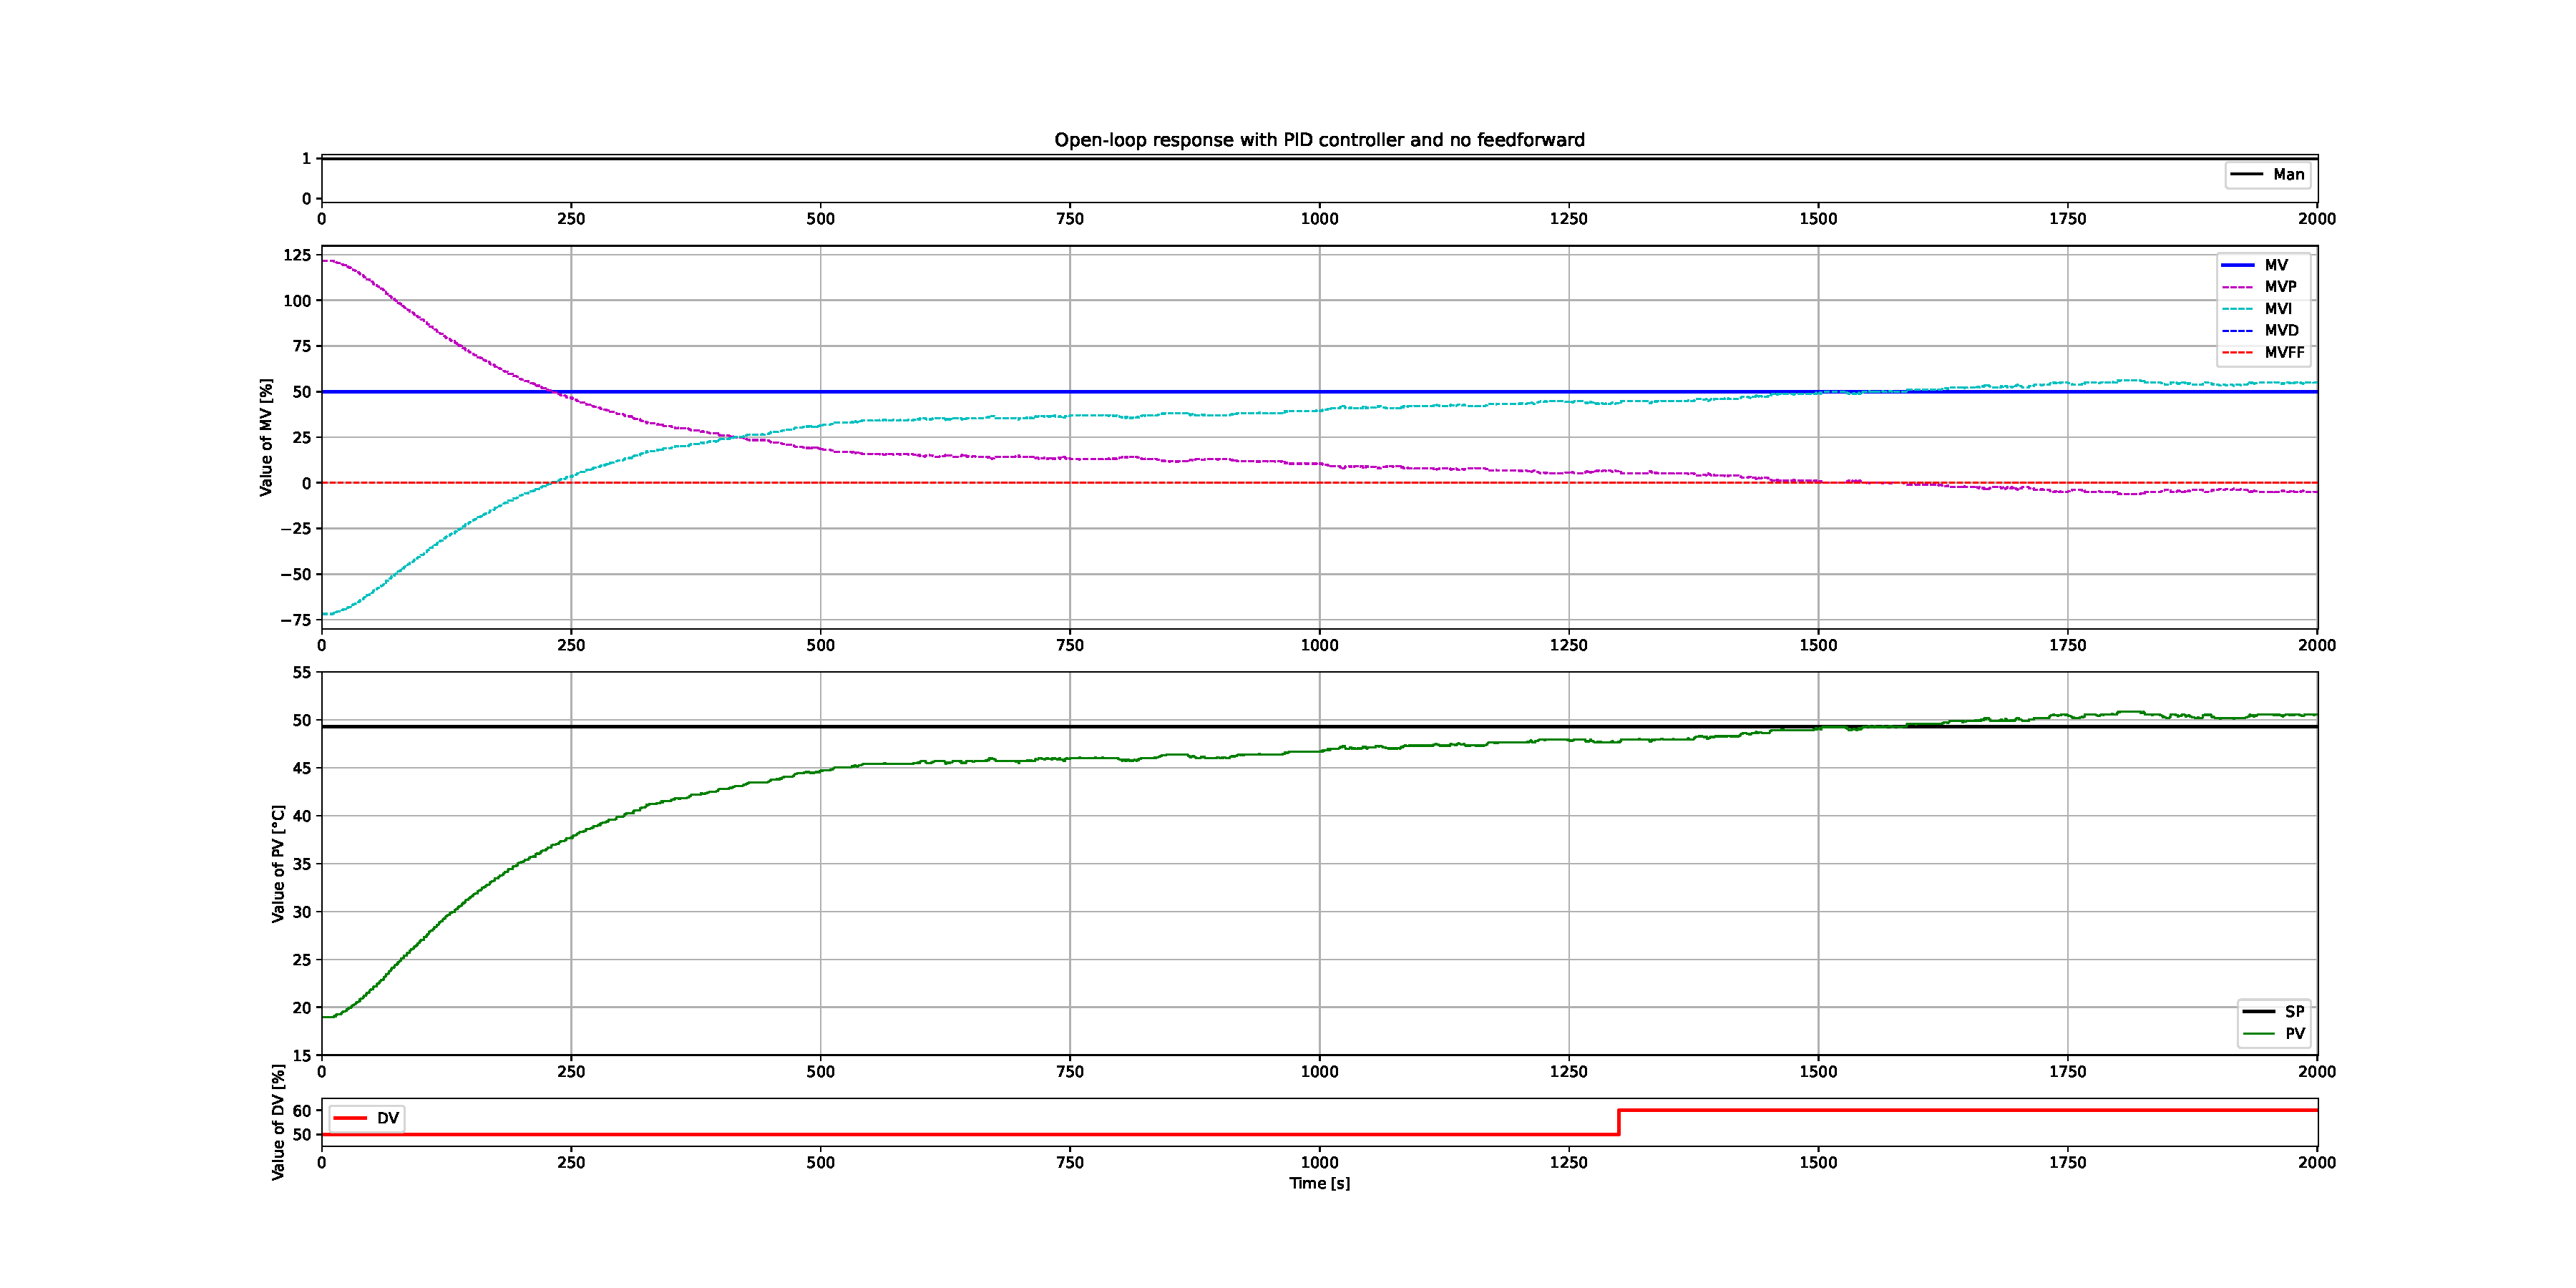
\includegraphics[width=1\textwidth]{../Plots/Experiment_scenario_2_2024-03-30-20h20.pdf}
	\caption{Données expérimentales du $1^{er}$ scénario}
	\label{fig:exp_scenario1}
\end{figure}
\begin{figure}[H]
	\centering
	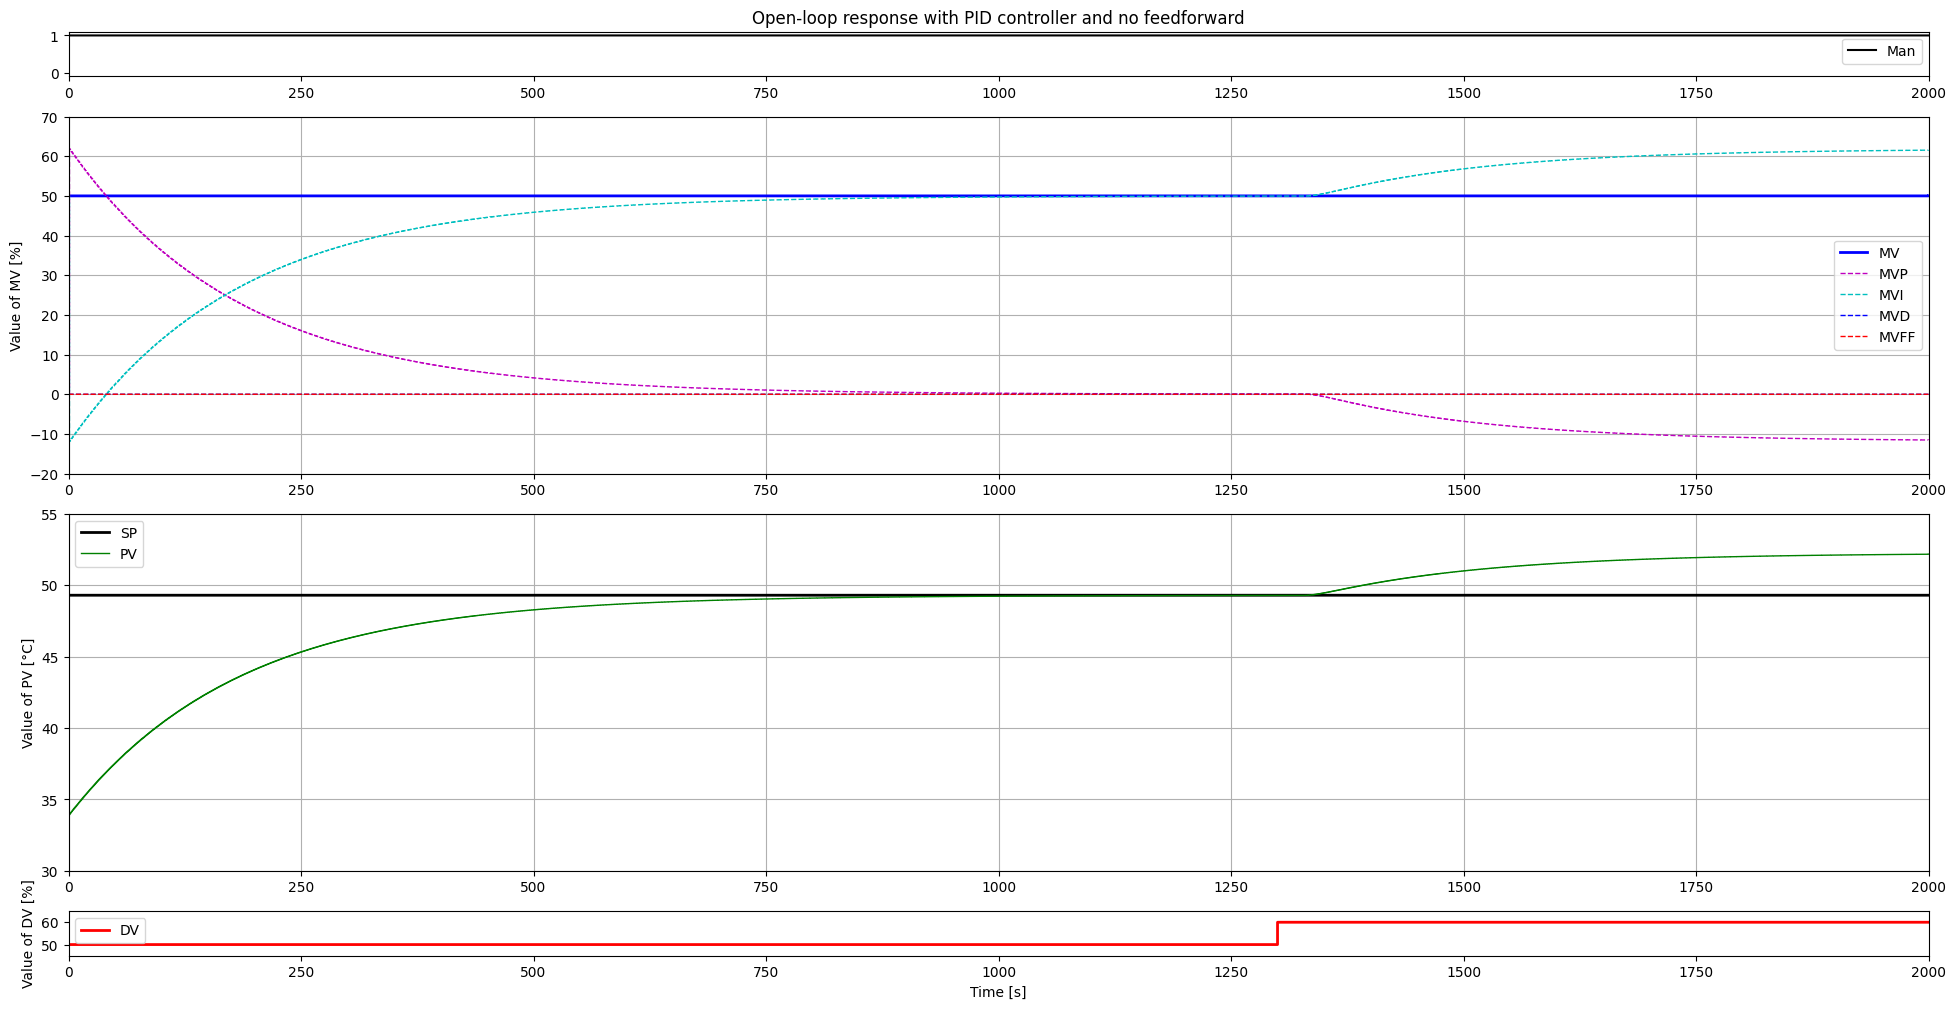
\includegraphics[width=0.8\textwidth]{figures/scenario2.png}
	\caption{Données de la simulation du $1^{er}$ scénario}
	\label{fig:sim_scenario1}
\end{figure}

On peut observer que le $PV$ n'a pas atteint la valeur de consigne ($SP$) avant le step de $10\%$ sur $DV$. Cela est dû au fait que, pour l'expérience,
la valeur du $PV$ à $t = 0s$ est de $\sim 18\degree C$ tandis que pour la simulation, il est de $\sim 34\degree C$. Néanmoins, une fois le step de $10\%$ sur $DV$ effectué,
la valeur du $PV$ converge jusqu'à la valeur de consigne et la dépasse à $t = 1500s$ ce qui correspond à un retard par rapport à la simulation $\sim \Delta t = 75s$. 
\\Une autre observation importante concerne la forme de la courbe $PV$ qui suggère un comportement typique d'un système du second ordre. Cependant, l'analyse des dynamiques du système 
lors du $1^{er}$ laboratoire avait révélé une seconde constante de temps très faible, $T_2P \sim 10^{-12}$. $T_{2P}$ étant négligeable, nous avions conclu que notre système se comportait
plutôt comme un système du premiere ordre en réponse à un changement sur $MV$. Selon nous, une des causes de ce changement de forme de courbe serait la température plus basse de la pièce qui affecterait 
l'inertie thermique du capteur de température. L'humidité de la pièce pourrait aussi être facteur puisque celle-ci affecte la conductivité thermique de l'air 
ambiant et donc pourrait aussi impacter l'inertie thermique du capteur.

\subsection{Scénario 2}

\begin{figure}[H]
	\centering
	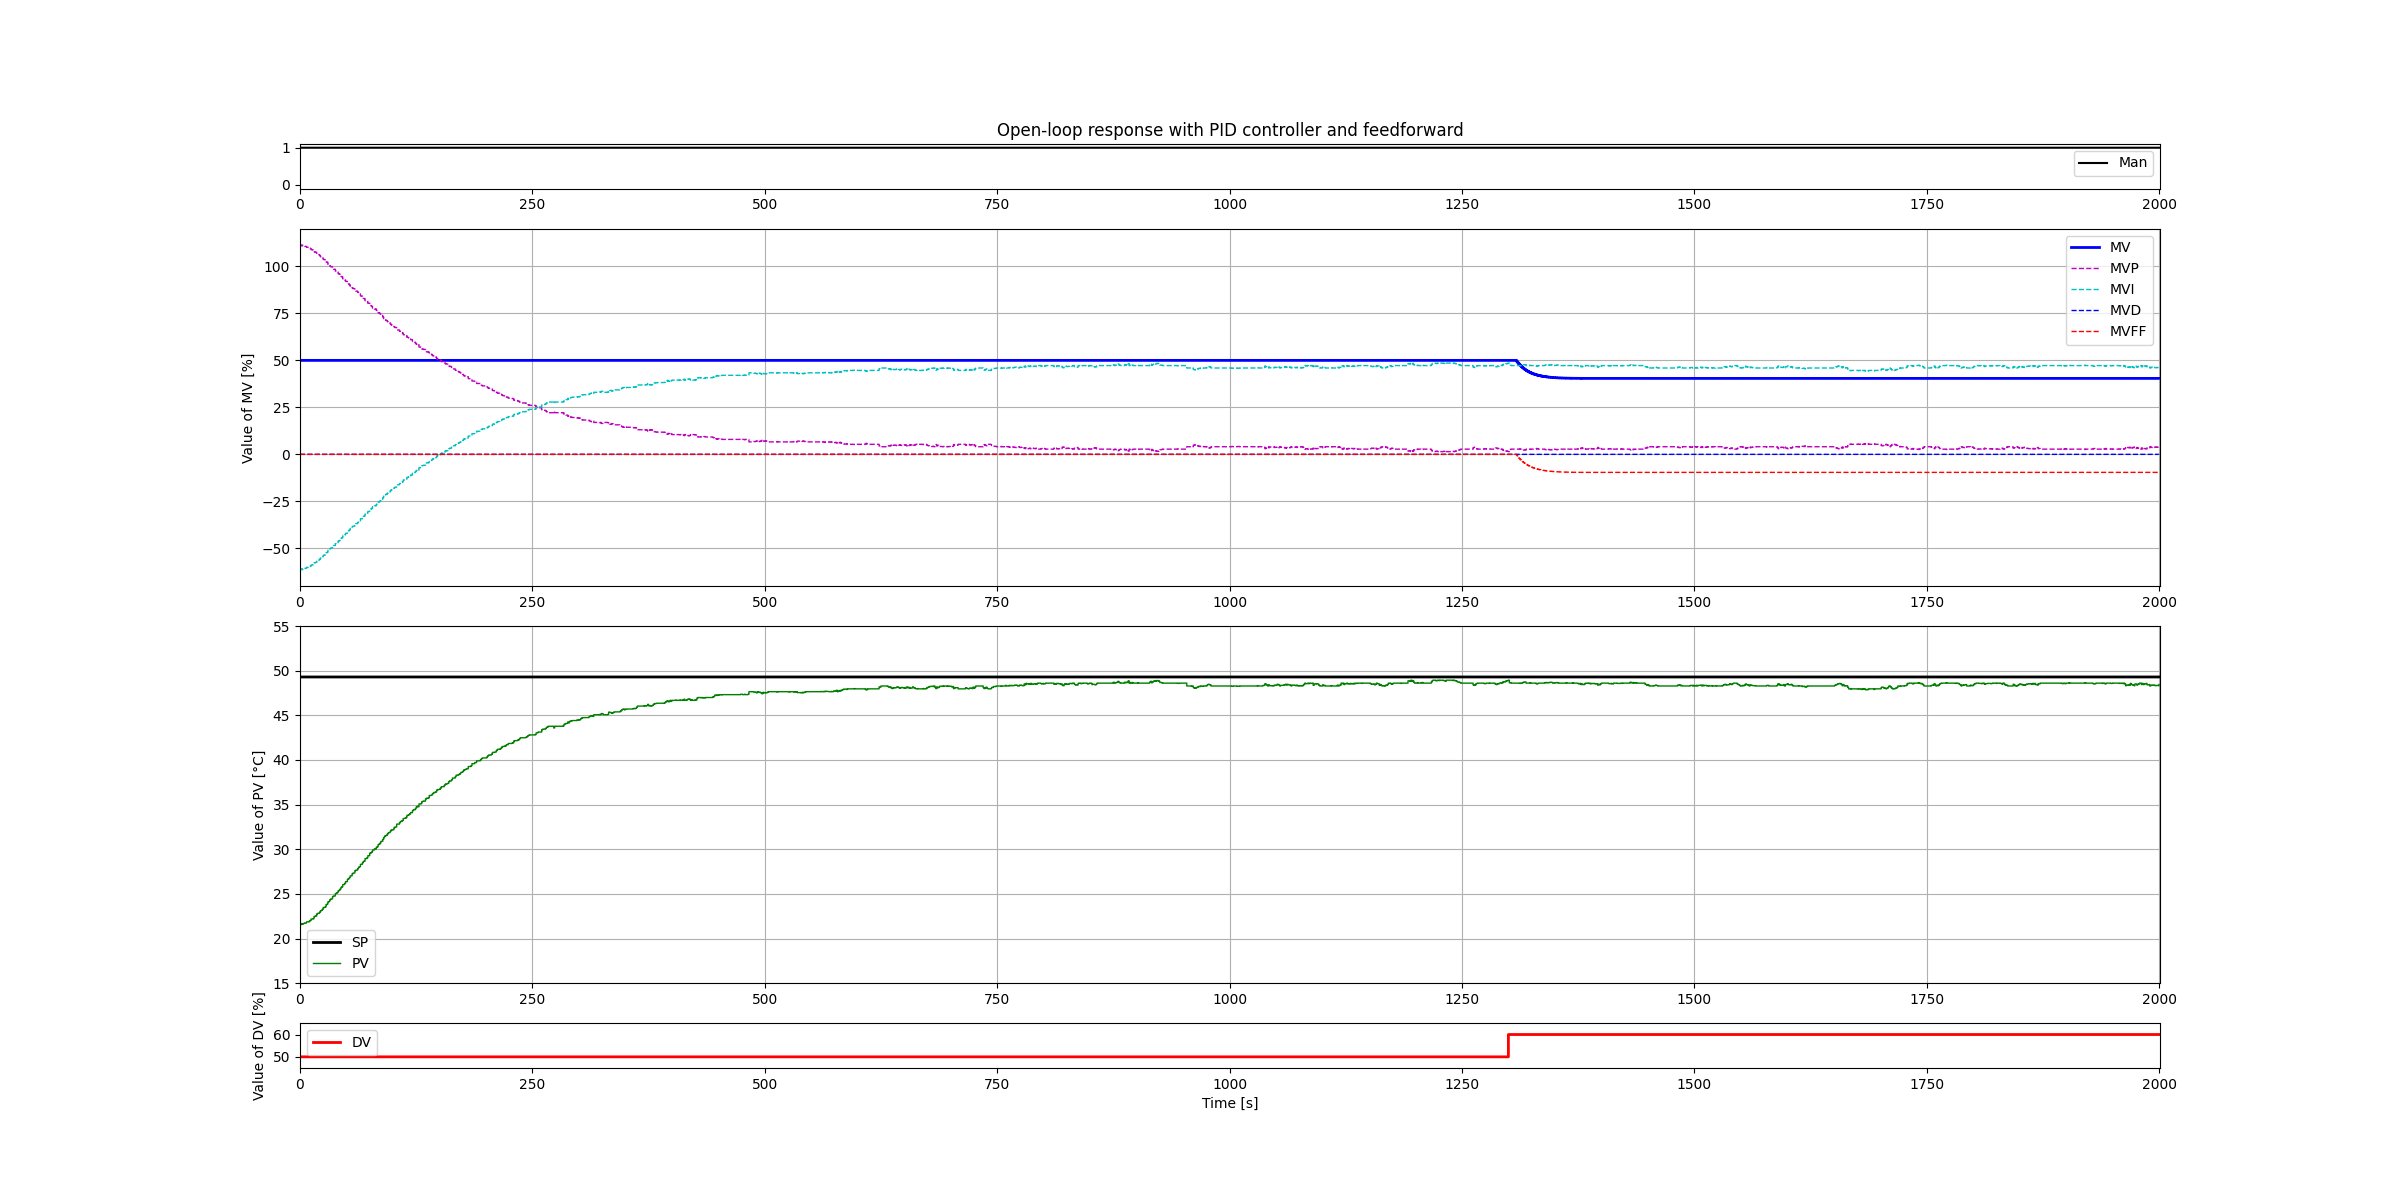
\includegraphics[width=1\textwidth]{../Plots/Experiment_scenario_3_2024-03-30-19h18.png}
	\caption{Données expérimentales du $2^{ème}$ scénario}
	\label{fig:exp_scenario2}
\end{figure}
\begin{figure}[H]
	\centering
	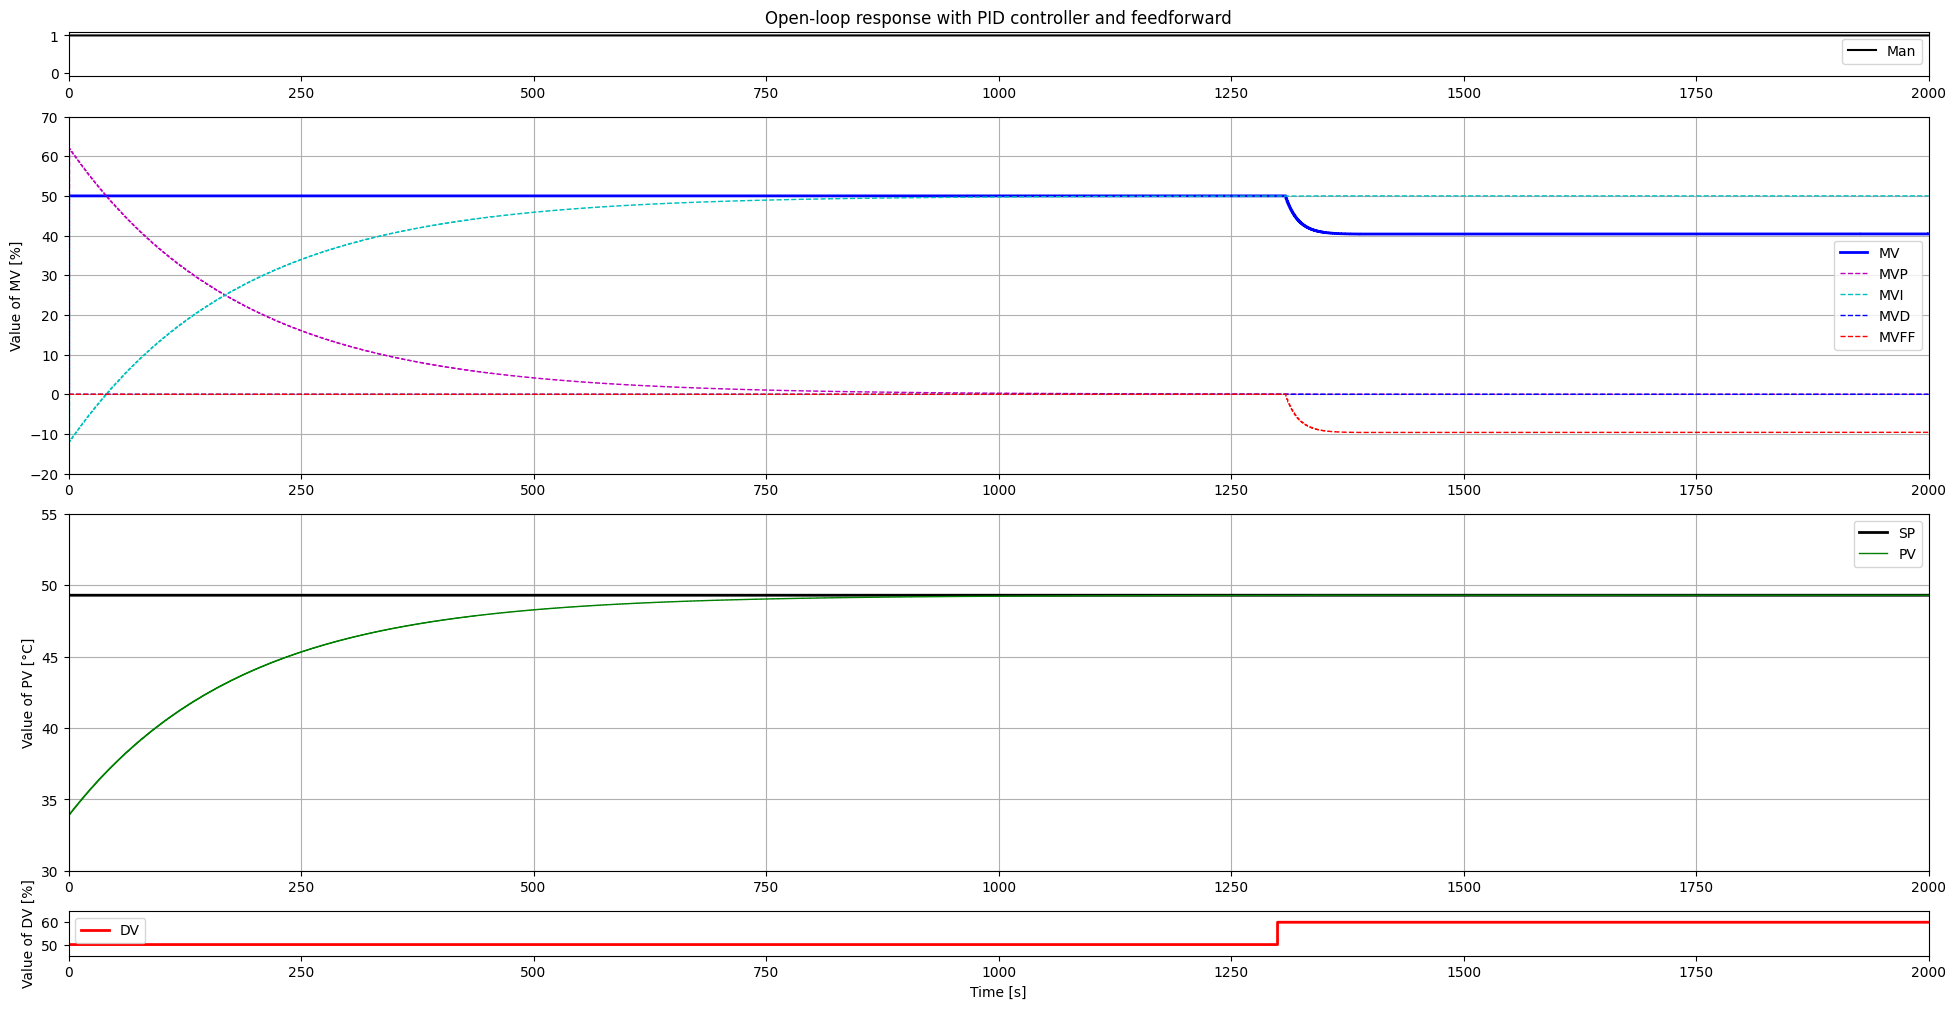
\includegraphics[width=0.8\textwidth]{figures/scenario3.png}
	\caption{Données de la simulation du $2^{ème}$ scénario}
	\label{fig:sim_scenario2}
\end{figure}

Dans ce scénario, tout comme dans le précédent(\ref{fig:exp_scenario1}), le système réagit plutôt comme un système du second ordre.
\\Toutefois, à la différence du scénario précédent, la valeur du $PV$ atteint à peu près au même moment la valeur de consigne ($SP$) que pour la simulation. Ceci est dû au fait
que la température du capteur n'a pas suffisamment pu redescendre entre les deux scénarios. En effet, la valeur de $PV$ à $t = 0s$ est de $\sim 22\degree C$ ce qui correspond 
à $4\degree C$ de plus que pour le scénario précédent. 
\\Mis à part ce détail, le système a bien répondu à la perturbation. L'utilisation du FeedForward a permis de neutraliser complètement l'effet du step de $10\%$ sur $DV$.

\subsection{Scénario 3}

\begin{figure}[H]
	\centering
	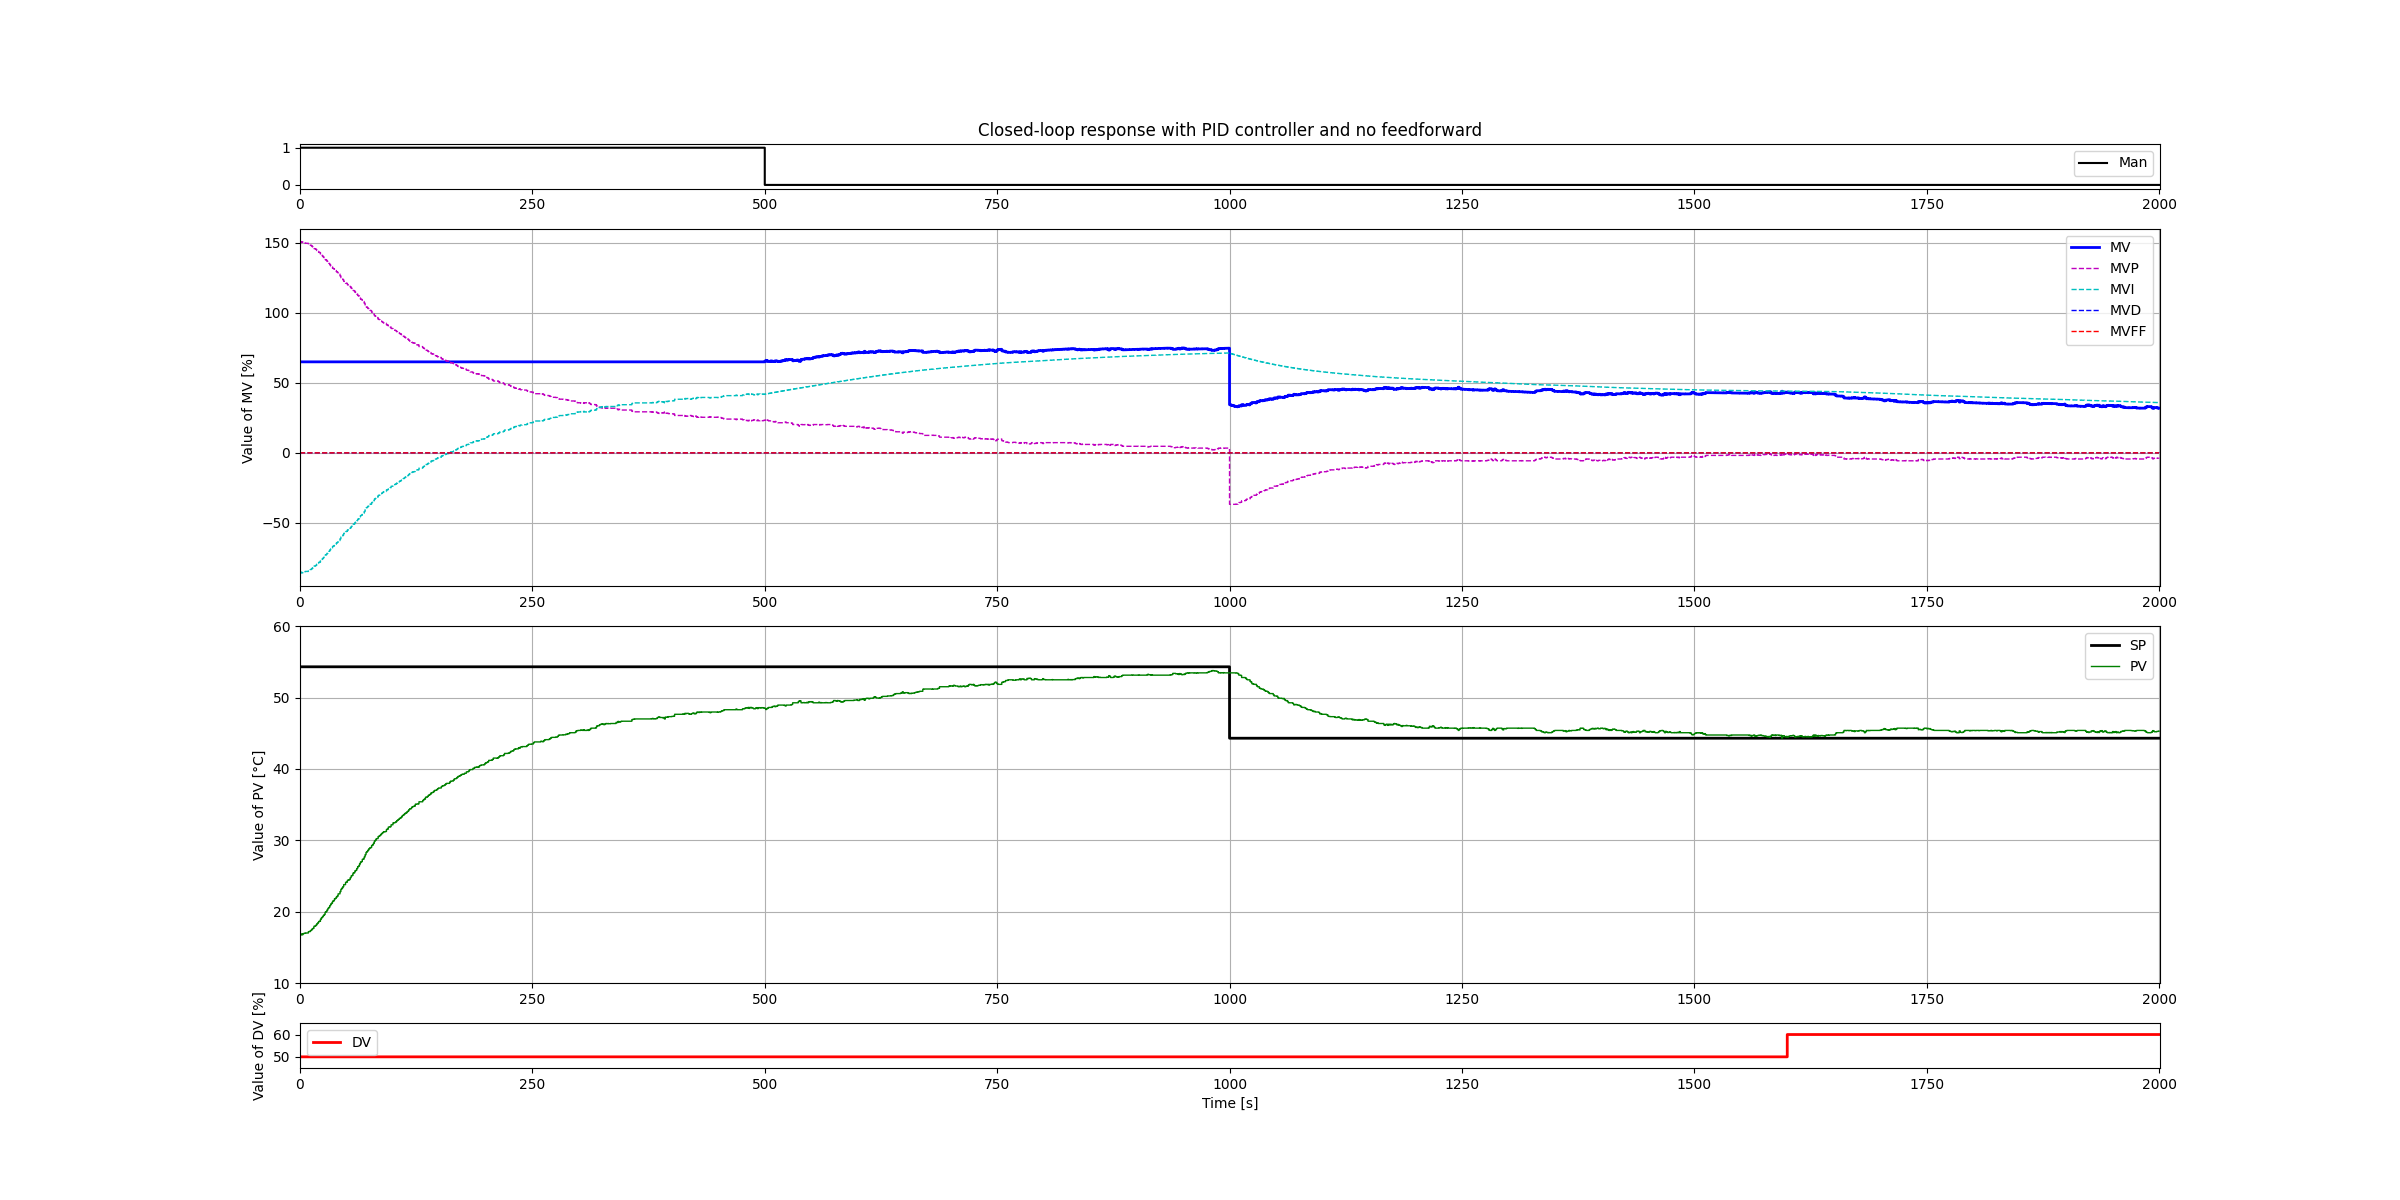
\includegraphics[width=1\textwidth]{../Plots/Experiment_scenario_5_2024-03-30-15h32.png}
	\caption{Données expérimentales du $3^{ème}$ scénario}
	\label{fig:exp_scenario3}
\end{figure}
\begin{figure}[H]
	\centering
	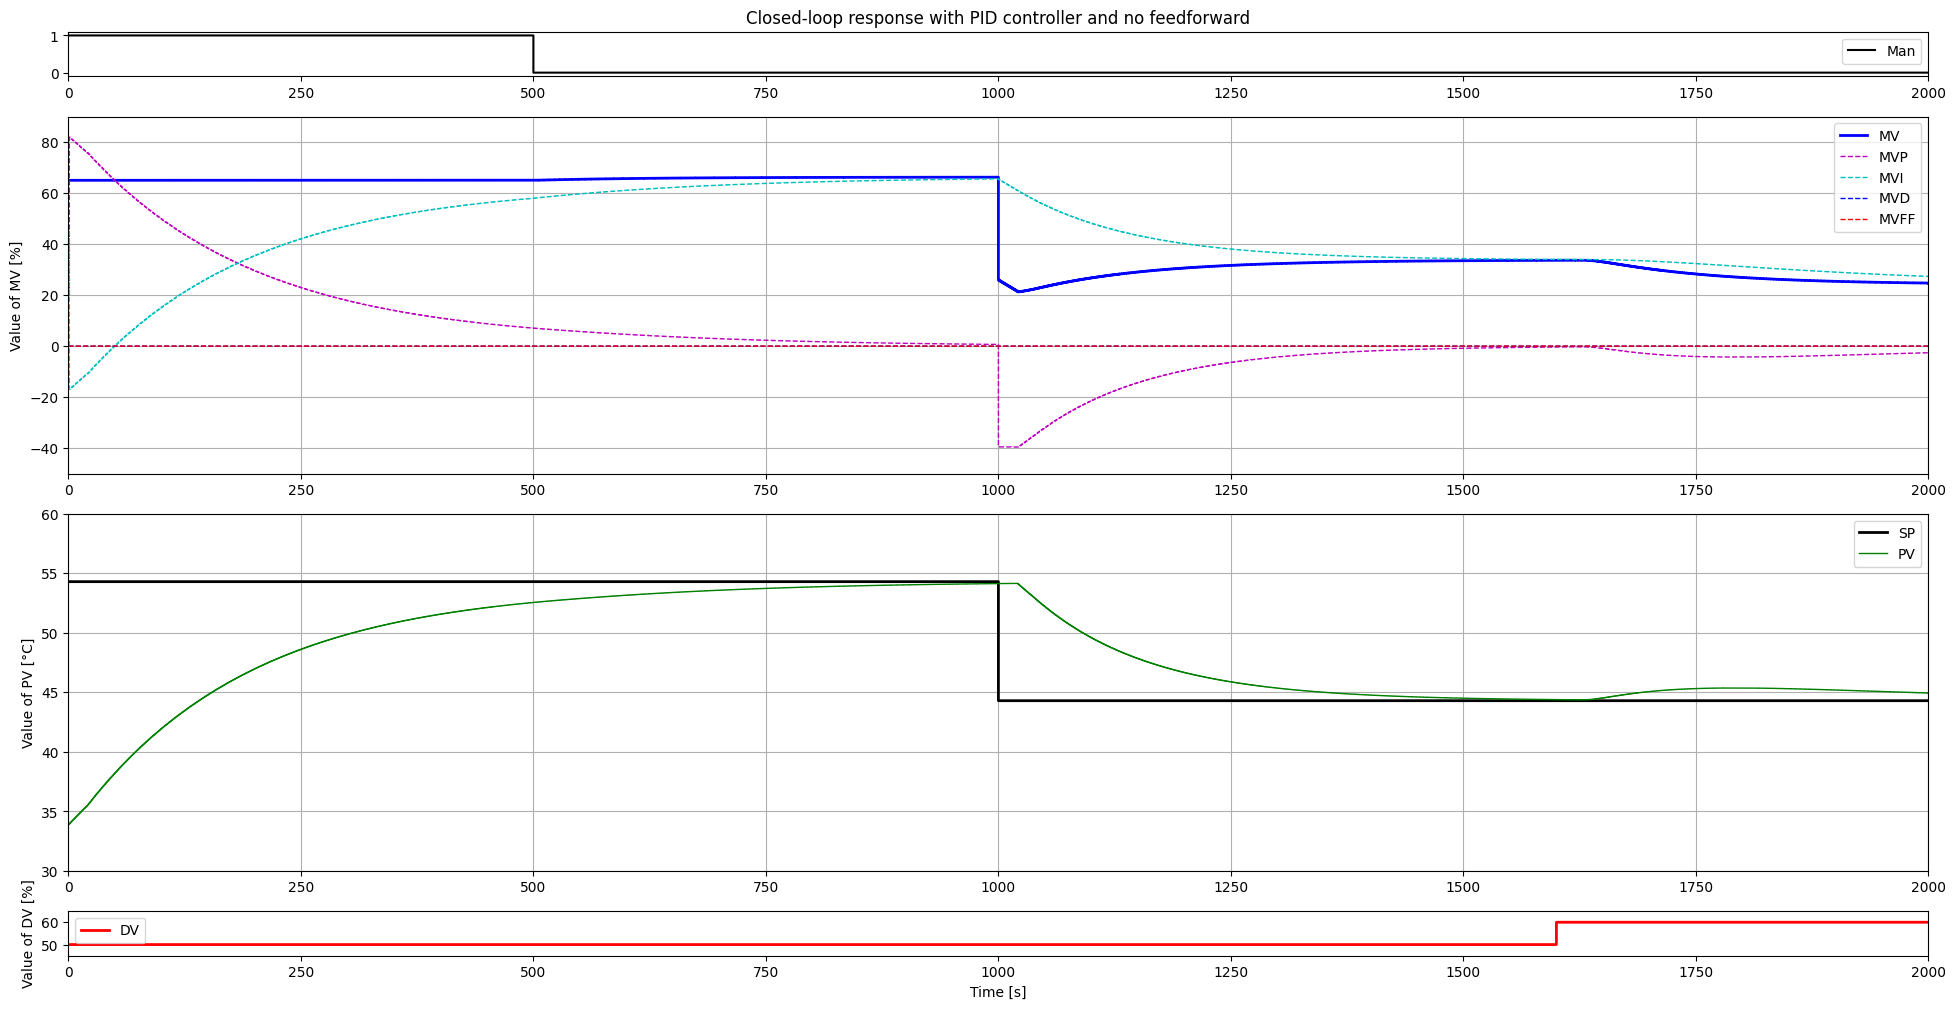
\includegraphics[width=0.8\textwidth]{figures/scenario5.png}
	\caption{Données de la simulation du $3^{ème}$ scénario}
	\label{fig:sim_scenario3}
\end{figure}

Comme pour le $1^{er}$ scénario (\ref{fig:exp_scenario1}), la valeur du $PV$ pour $t = 0s$ est de $\sim 17\degree C$ ce qui cause un retard, par rapport à la simulation, dans l'atteinte de la valeur
de consigne. Ensuite, on observe que le régulateur PID réagit correctement au step de $-10\%$ et atteint la nouvelle valeur de consigne presque en même temps que
pour la simulation. Pour finir, après la perturbation, on observe bien une diminution de $MV$ afin de faire revenir $PV$ à la valeur de consigne. 

\subsection{Scénario 4}

Pour ce scénario, nous avons décidé de répéter l'expérience en changeant la valeur du gamma suite à l'observation de son impact sur les données expérimentales.
Cet impact n'est cependant pas visible sur la simulation.

\subsubsection{$\gamma = 0.5$}

\begin{figure}[H]
	\centering
	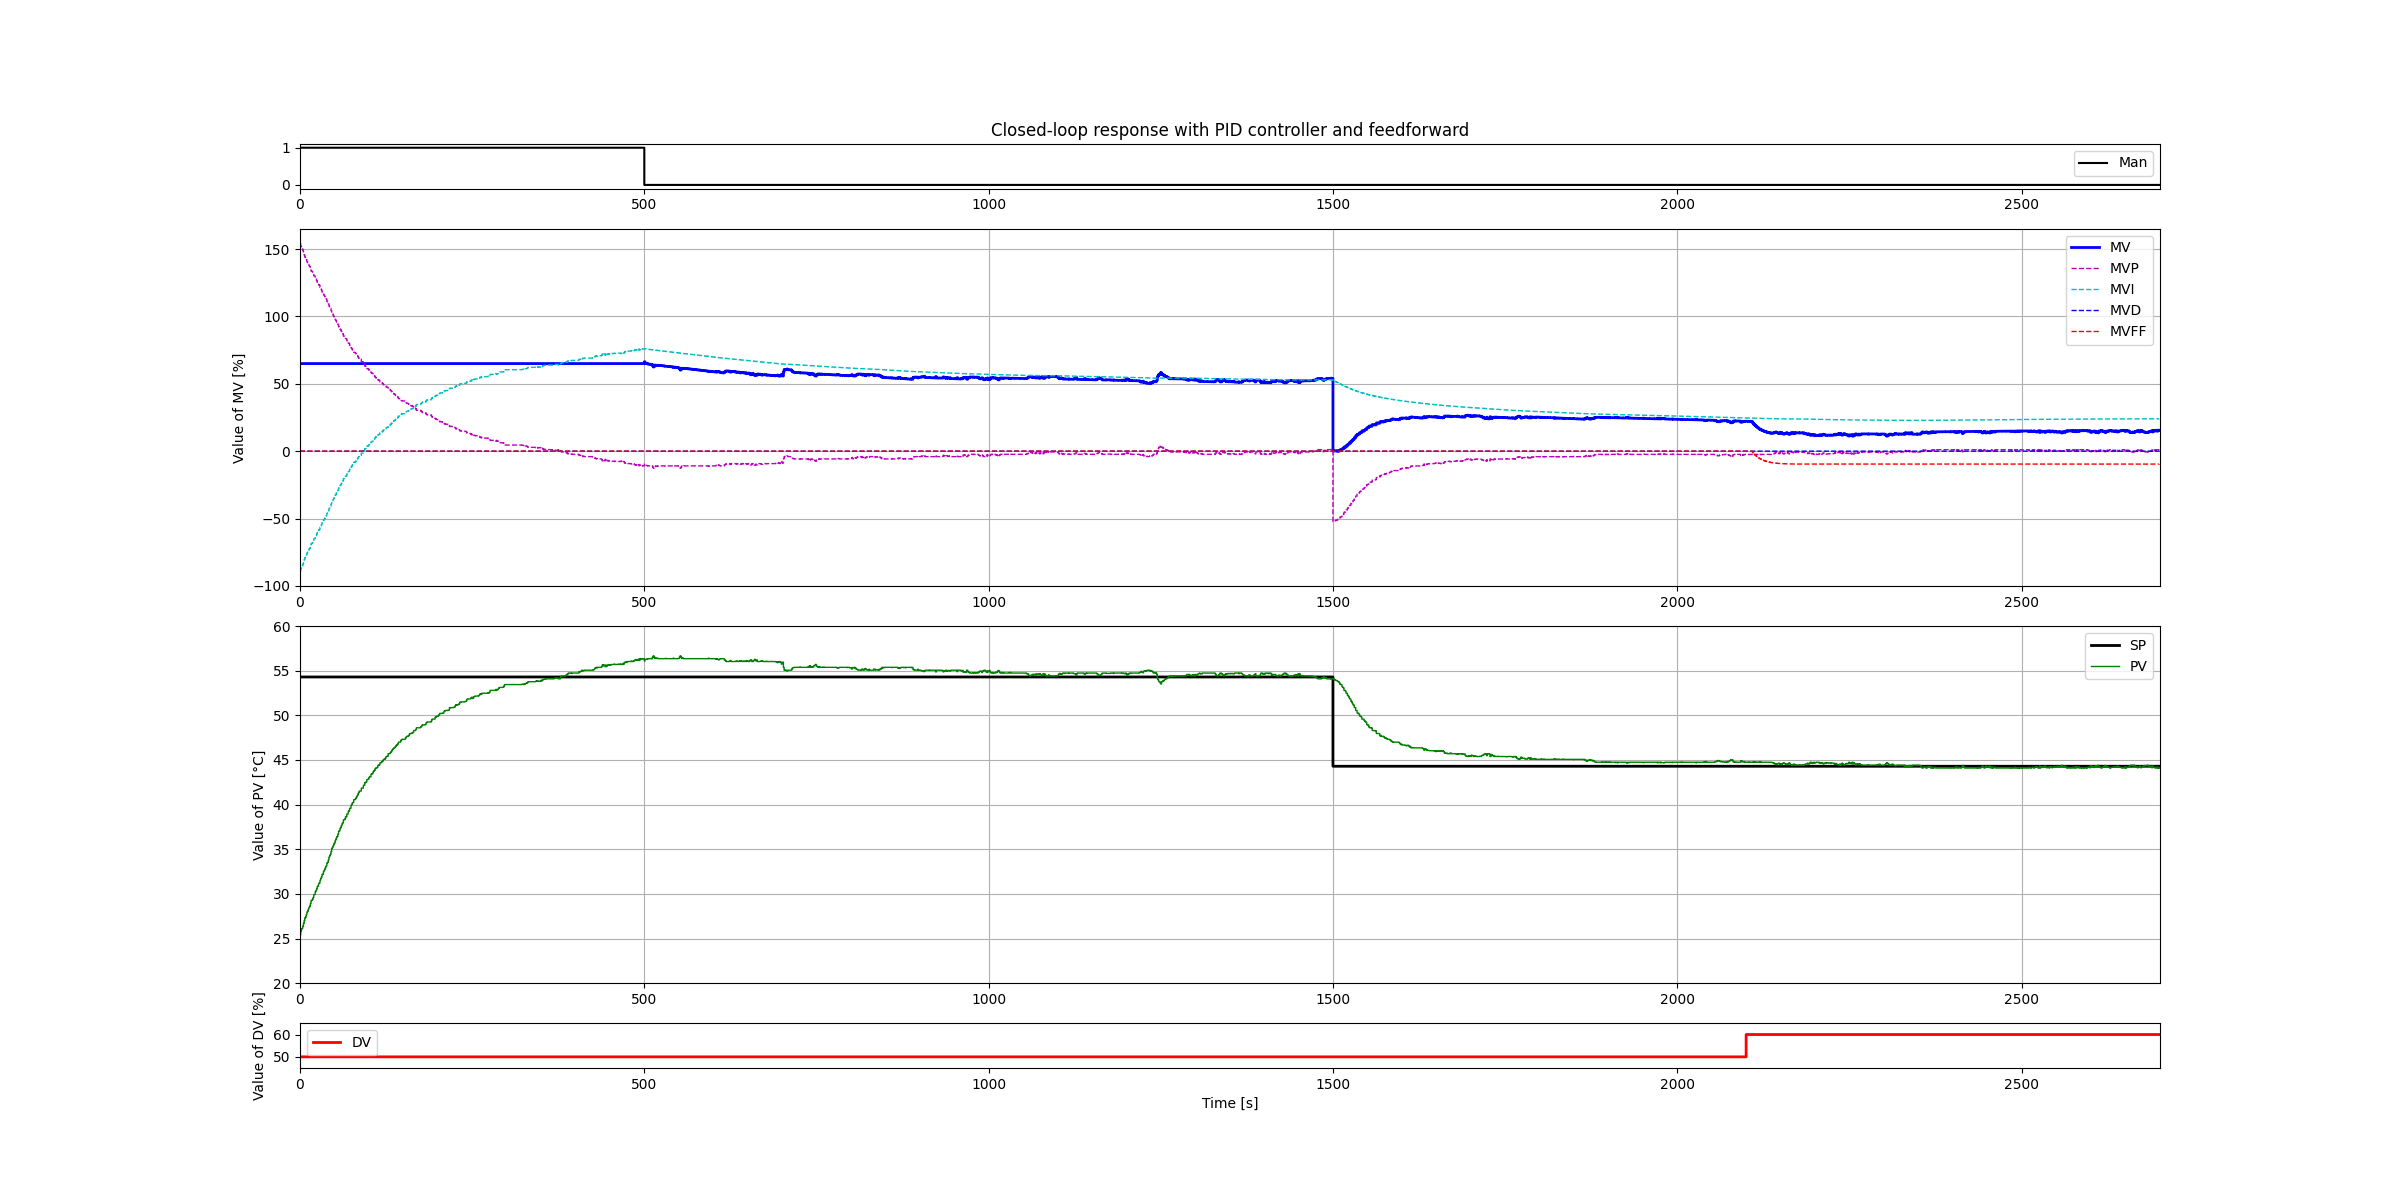
\includegraphics[width=1\textwidth]{../Plots/Experiment_scenario_7_2024-03-29-17h44.png}
	\caption{Données expérimentales du $4^{ème}$ scénario, $\gamma = 0.5$}
	\label{fig:exp_scenario5_0.5}
\end{figure}
\begin{figure}[H]
	\centering
	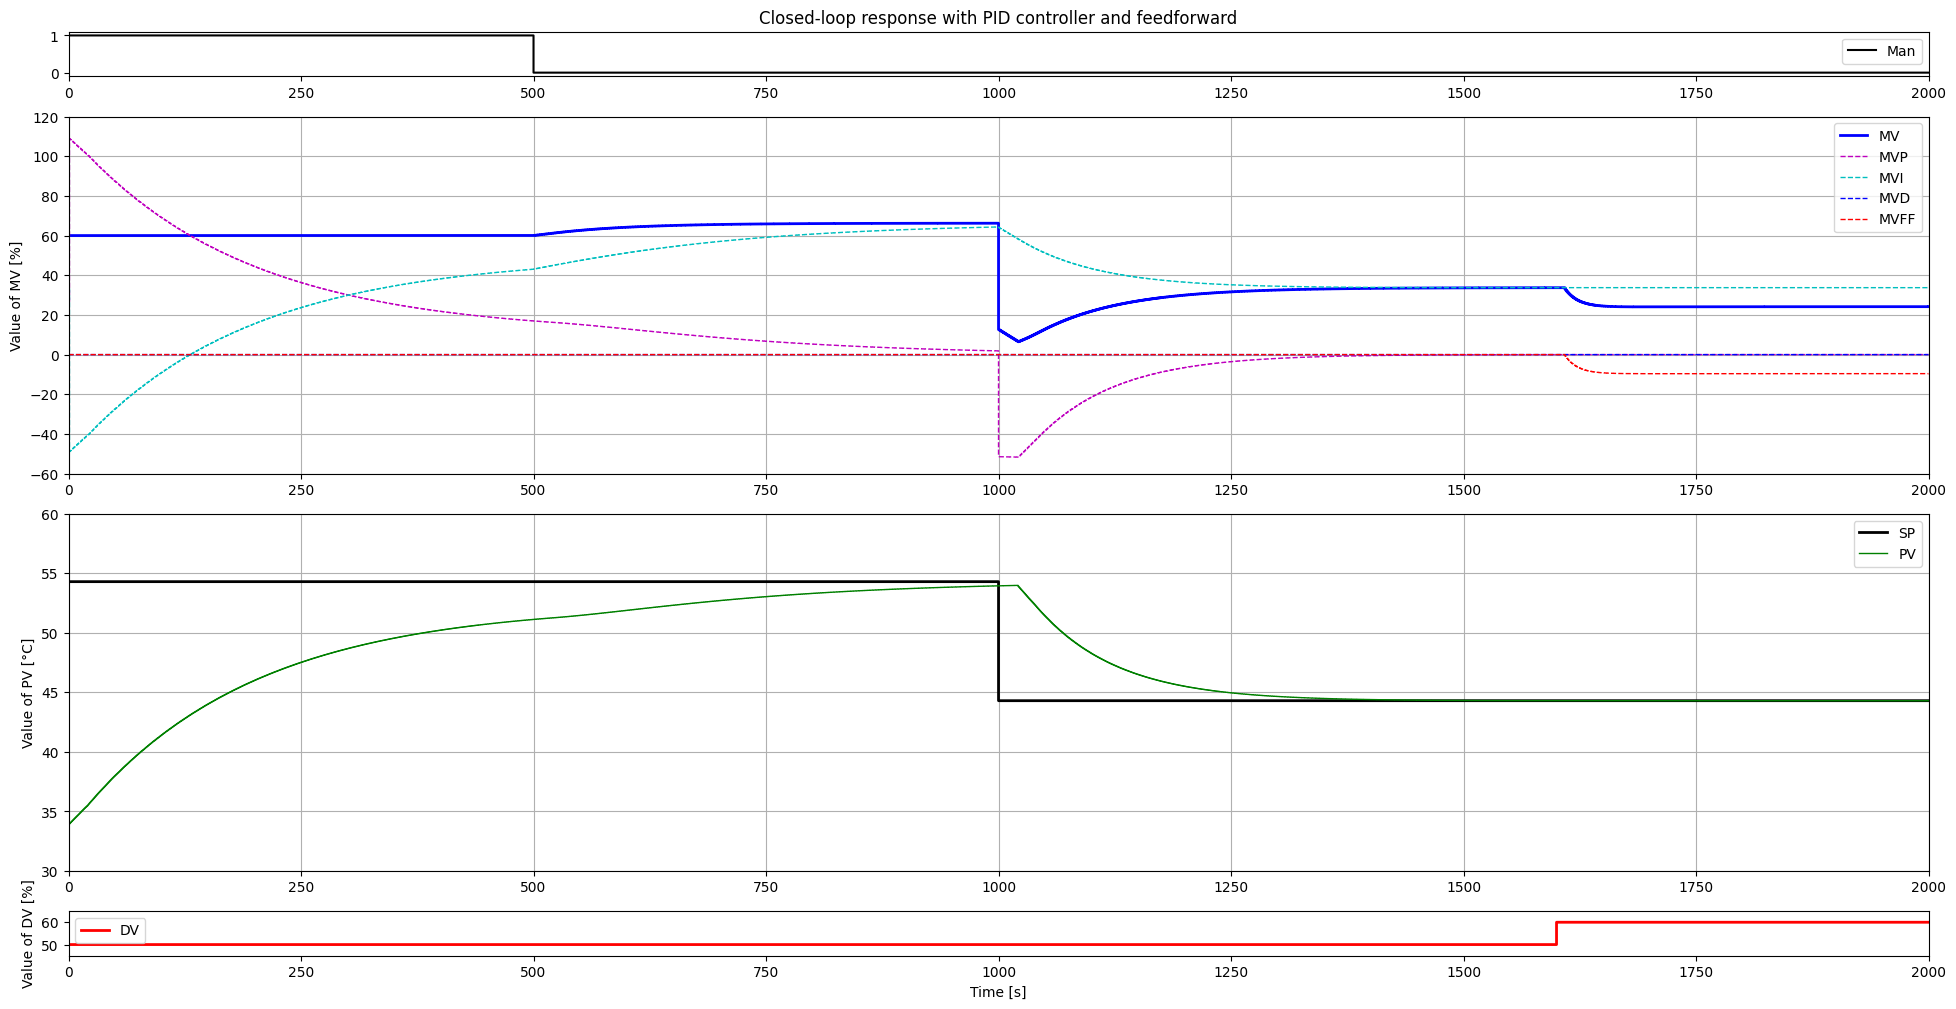
\includegraphics[width=0.8\textwidth]{figures/scenario7.png}
	\caption{Données de la simulation du $4^{ème}$ scénario, $\gamma = 0.5$}
	\label{fig:sim_scenario5_0.5}
\end{figure}

Premièrement, la valeur de $PV$ à $t = 0s$ étant plus élevée que pour tous les scénarios précédents, on observe une convergence de $PV$ vers la valeur de consigne 
plus rapide. Le système présente également un comportement plus proche d'un système du $1^{er}$ ordre. 
\\Par ailleurs, contrairement à ce qui est observé dans la simulation, l'expérience montre un dépassement (overshoot) de la température.
La forme de la courbe de l'expérience diffère beaucoup de celle de la simulation. Cela n'est pas dû à la valeur de gamma puisque l'overshoot aurait alors été également visible dans la simulation. 
L'occurence de l'overshoot dans l'expérience, mais pas dans la simulation ainsi que la grande similitude entre les données expérimentales et simulées dans le 
scénario suivant, suggèrent que cet overshoot pourrait résulter d'une erreur de manipulation lors de l'expérience.
\\Outre l'overshoot, on observe que le régulateur PID réagit correctement à la perturbation puisque $PV$ reste constant malgré le step de $10\%$ sur $DV$.

\subsubsection{$\gamma = 0.7$}

\begin{figure}[H]
	\centering
	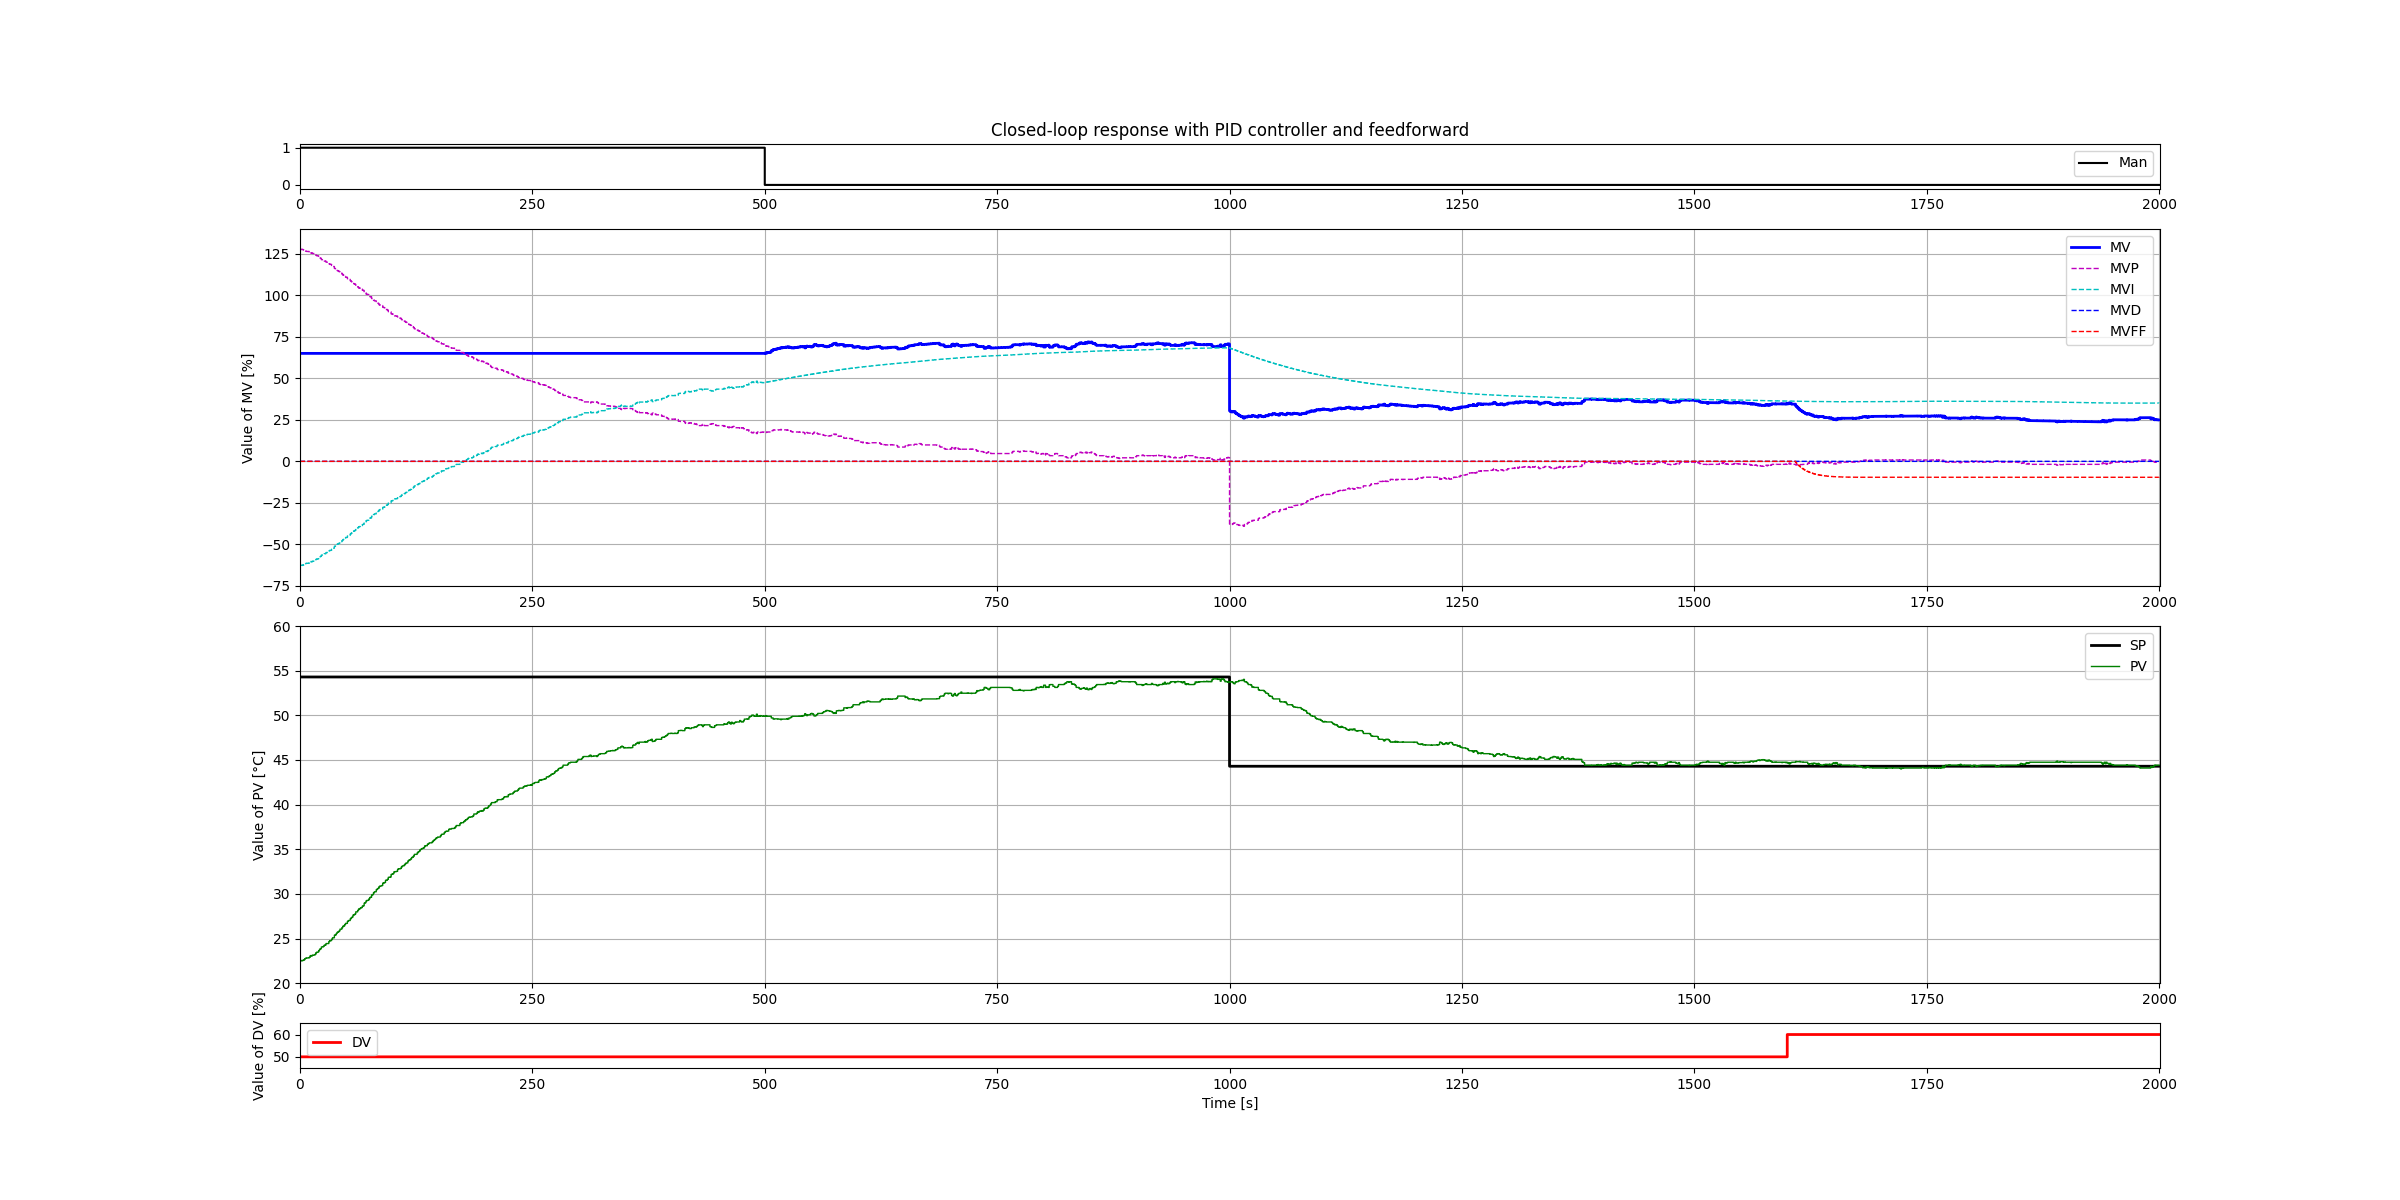
\includegraphics[width=1\textwidth]{../Plots/Experiment_scenario_7_2024-03-29-22h23.png}
	\caption{Données expérimentales du $4^{ème}$ scénario, $\gamma = 0.7$}
	\label{fig:exp_scenario5_0.7}
\end{figure}
\begin{figure}[H]
	\centering
	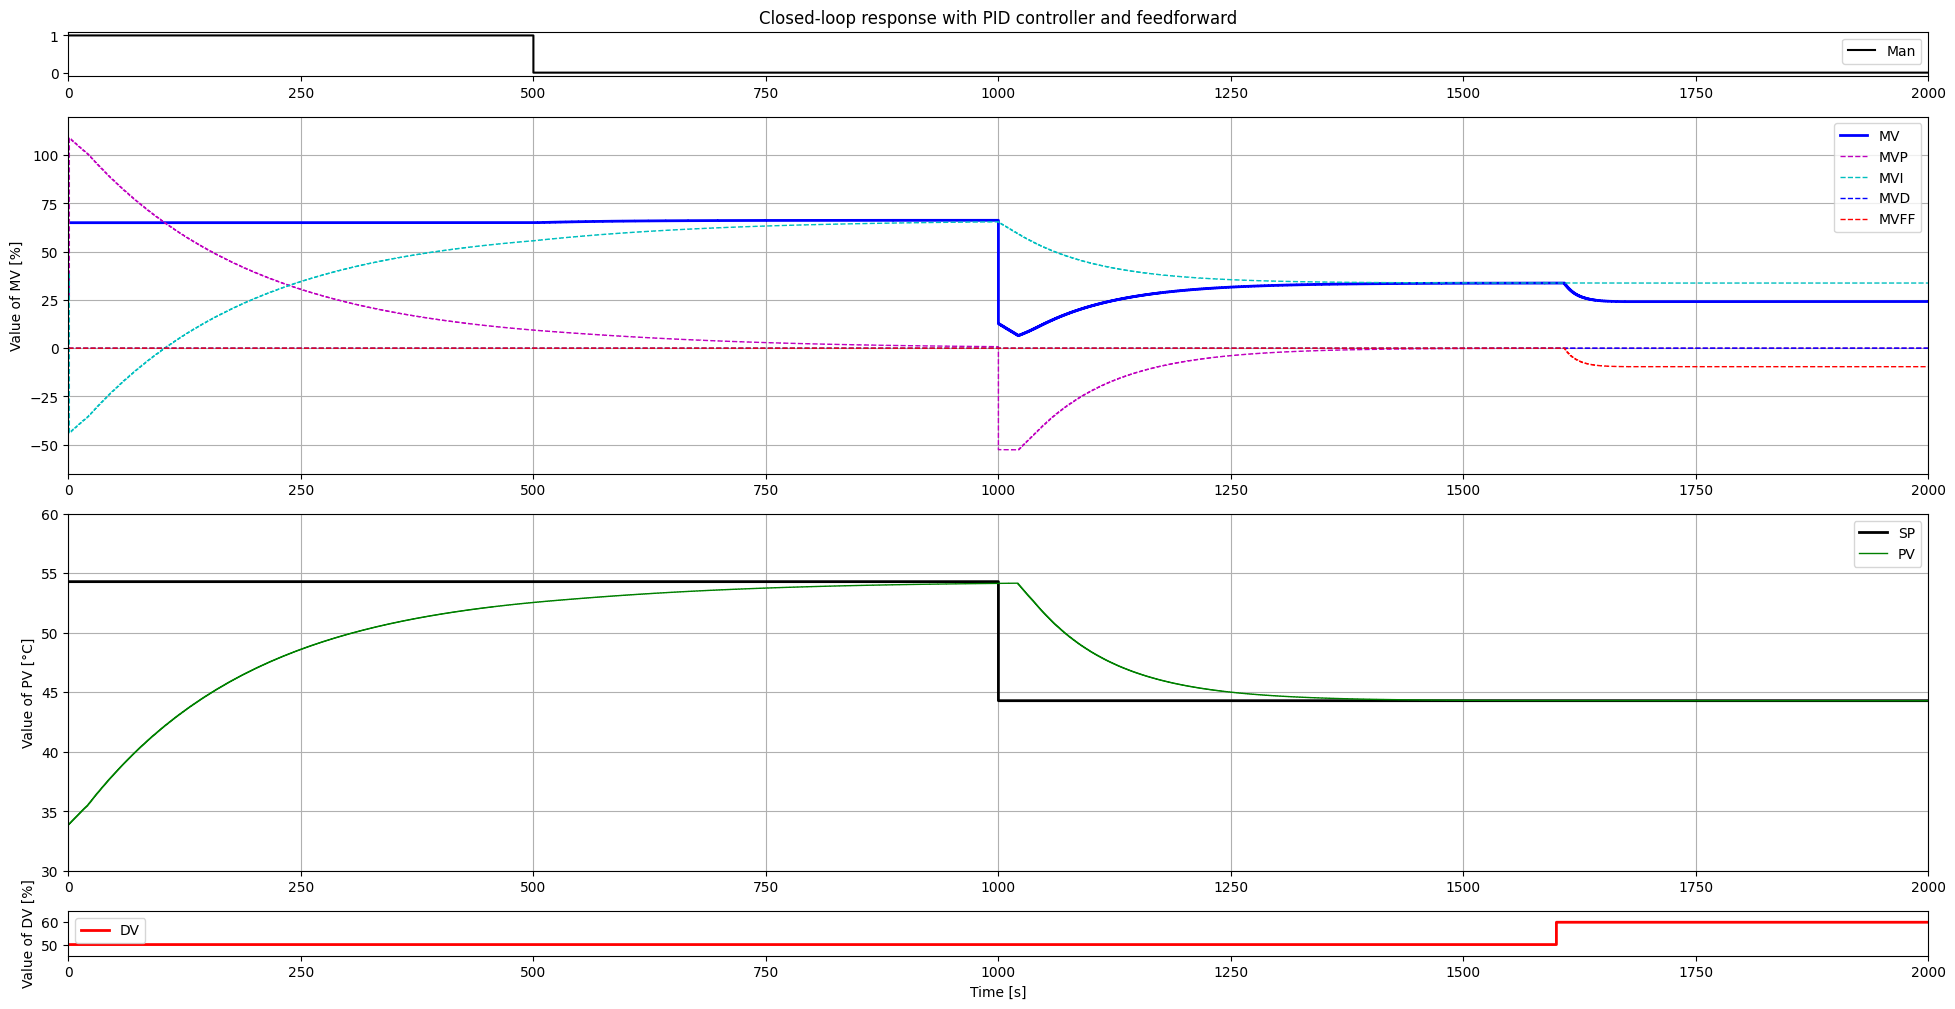
\includegraphics[width=0.8\textwidth]{figures/scenario77.png}
	\caption{Données de la simulation du $4^{ème}$ scénario, $\gamma = 0.7$}
	\label{fig:sim_scenario5_0.7}
\end{figure}

Pour cette dernière expérience, on observe des résultats beaucoup plus cohérents pr rapport à la simulation. Le système réel prend plus de temps à converger
vers la consigne ce qui est dû à la valeur initiale de $PV$ comme discuté précédemment. L'overshoot observé dans le scénario précédent n'est plus présent.
L'augmentation de $\gamma$ peut y avoir contribué puisque cela a comme effet de diminuer ``l'agressivité'' du régulateur en diminuant la constante de gain $K_c$ de celui-ci.
\\Le régulateur PID réagit correctement au changement de consigne et atteint la nouvelle valeur presque en même temps que pour la simulation. 
On peut justement observer l'influence du gamma en comparant ce changement de consigne avec celui où $\gamma = 0.5$ (\ref{fig:exp_scenario5_0.5}). En effet,
la courbe de $PV$ est plus progressive pour $\gamma = 0.7$ que pour $\gamma = 0.5$. Ceci est dû à la diminution de $K_c$ : 
\begin{equation}
	T_{CLP} = \gamma\cdot T_{1P}
	K_c = \frac{1}{K}\,\frac{T_{1P}+T_{2P}}{T_{CLP}+\theta}
\end{equation}
Et cette diminution de $K_c$ a pour effet de diminuer la valeur de $MV$ à chaque itération du régulateur PID et donc de rendre la réponse du système plus lente.
Pour terminer, le régulateur réagit correctement à la perturbation causée par le step de $10\%$ sur $DV$ puisque, comme pour la simulation, $PV$ reste constant.
